
\subsubsection{Methodology.}

\( k \)-Nearest neighbours (\( k \)-NN) is a simple, distance-based machine learning classification algorithm that lazily learns its class based on the majority class (for classification) or average value (for regression) of its nearest peers.

Due to \( k \)-NN's 'distance-based' nature, categorical features cannot be directly interpreted, hence they need to be transformed to numerical vectors. As in the dataset, most of the variables are numerical or ordinal values, the data is fed into the algorithm \textit{per se}, i.e., by \textit{label encoding}.

Another factor to be concerned of is feature scaling, as different measurements are made in different scales. Two scaling methods are tested: \textit{Normalisation}, where each feature is mapped to the range \( [0, 1] \) via a min-max transformation:

\begin{align*}
    \mathbf{x} \mapsto \frac{\mathbf x - \min\mathbf x}{\max\mathbf x - \min\mathbf x}
\end{align*}

and \textit{Box-Cox + Standardisation}, where each feature is fed to a Box-Cox transformation with its according optimal parameter \( \lambda \) (if applicable), then standardised:

\begin{align*}
    \mathbf{x} 
        \mapsto \mathbf{x'} := \frac{\mathbf{x}^\lambda - 1}\lambda  
        \mapsto \frac{\mathbf x' - \overline{\mathbf x'}}{\mathrm{std\ }\mathbf x'}
\end{align*}

\subsubsection{Experiments \& Results.}

\begin{table}[h]
    \centering
    \begin{tabular}{ccc}
        \toprule
        TPR, \( 19 \)-NN
        & \textbf{Full}
        & \textbf{Simplified\footnotemark{}}
        \\
        \midrule
        \textbf{Normalisation}
        & \( 86.274\% \)    
        & \( 88.697\% \)
        \\
        \midrule
        \textbf{Box-Cox + Standardisation}
        & \( 90.184\% \)    
        & \( 93.188\% \)
        \\
        \bottomrule
    \end{tabular}
    
    \raggedright
    \( ^1 \) {\small \texttt{fbs}, \texttt{bp} and \texttt{chol} are excluded from the model}
    
    \centering
    \vspace{4pt}
    \caption{\centering TPR performance of \( k \)-NN models, where \( k = 19 \)}
\end{table}

A total of four models are tested on a various range of values for \( k \in [3, 50]\), with a label cutoff at \( \delta = 0.5 \). It is observed that the simplified model with Box-Cox transformation followed by standardisation performed the best, with \( \text{TPR} = 93.94\% \) saturated at \( k \ge 19 \). 

\begin{figure}[H]
    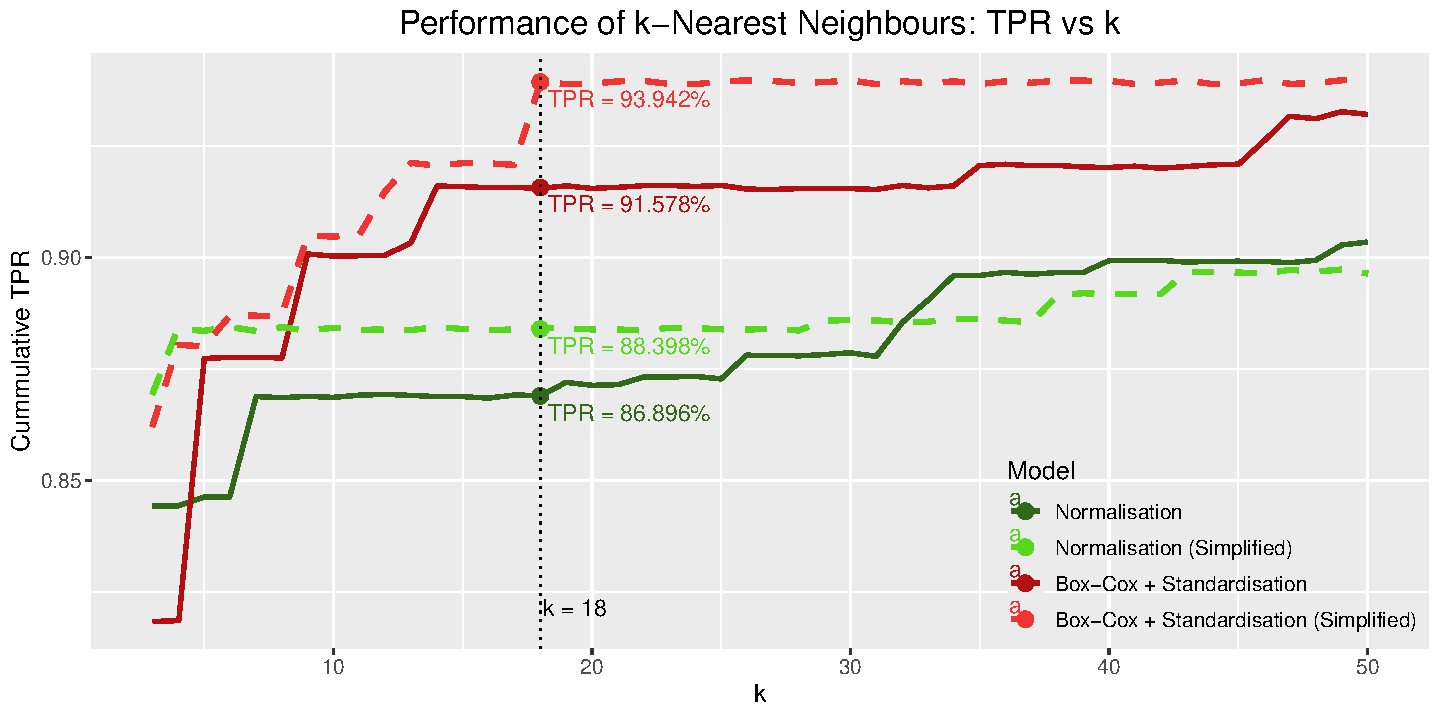
\includegraphics[width=\linewidth]{31.kNN.pdf}
    \caption{\centering TPR performance of \( k \)-NN models with running \(k\)}
\end{figure}
    
Generally, standardisation methods outperform normalsation as the best preprocessing method for \( k \)-NN. In terms of model complexity, simple models fit best for small values of \( k \), however when \( k \) gets larger, then simple models fit the data worse compared to full models; this may rather shows the effect of underfitting than outperformance. By the elbow method, it can be seen that the best performing model is a \textbf{\( 19 \)-nearest neighbour model on a Box-Cox, standardised dataset}.